\section{Experiments on CTR Data}
In this section, we demonstrate that the proposed adaptive model is effective for CTR prediction. First, we compare our model with other state-of-art models on several real-world data sets. Then, we conduct further analysis on the proposed method. In particular, because the key in our proposed model is the threshold value, we show how to locate an optimal threshold value with exploration on the data set.

\subsection{Experimental Settings}
We evaluate the effectiveness of our proposed adaptive model on three data sets. Two data sets are from Kaggle competitions, while another is a data set from our production system.
\begin{enumerate}
\item Criteo Dataset:\footnote{Criteo Data Set: http://www.kaggle.com/c/criteo-display-ad-chanllenge} This data set originates from a Kaggle competition. We use the processed set used in \cite{Juan:2016:FFM:2959100.2959134}.\footnote{Criteo Data Set: https://www.csie.ntu.edu.tw/$\sim$cjlin/libsvmtools/datasets/binary.html} We randomly split the data to 74\% for training, 13\% for validation, and 13\% for testing.
\item Avazu Dataset:\footnote{Avazu Data Set:http://www.kaggle.com/c/avazu-ctr-prediction} This set is from another Kaggle competition and we again use the processed form in \cite{Juan:2016:FFM:2959100.2959134}.\footnote{Avazu Data Set: https://www.csie.ntu.edu.tw/$\sim$cjlin/libsvmtools/datasets/binary.html} We split the data to 77\% for training, 10\% for validation, and 13\% for testing.
\item Company Dataset: This data set is from our service of providing personalized advertisement recommendation. We collect several days of users' click records, and let the last two days be used for validation and testing.
\end{enumerate}

The statistics of all data sets are summarized in Table \ref{tab1}.

\begin{table}[ht]
\caption{Statistics of data sets. Some information of the company data is not revealed. Density is the percentage of non-zeros in the data.}
\label{tab1}
\centering
\begin{tabular}{|c|c|c|c|c|}
  %\toprule
   \hline
  Data Set & \#instances & \#features & \#fields & density \\
  \hline
  criteo & 45,840,617 & 1,000,000 & 39 & 0.0039\%  \\
  \hline
  avazu & 40,428,967 & 1,000,000 & 15 & 0.0015\%  \\
  \hline
  company &tens of millions & $\le$500,000   &tens & $\leq$0.0050\% \\
  %\bottomrule
  \hline
\end{tabular}
\end{table}

Following most studies on CTR prediction, we consider the following logistic loss as our evaluation criterion.
\begin{equation}
\text{logloss}=\frac1{m}\sum_{i=1}^{m} \log(1+\exp(-y_{i}\phi(\boldsymbol{w}, \boldsymbol{x}_{i}))).
\end{equation}

We compare four models discussed in this work, where Poly2, FM and FFM serve as baselines to be compared with the proposed adaptive model.

\subsection{Results of the Comparison}
\label{sec:comparition}

We follow a rigorous setting to select parameters. The search range of each parameter is given as follows.
\begin{itemize}
\item $\eta$: the learning rate is used in the stochastic gradient  implementation for each model. We consider $\eta$ in $\{0.05,0.1,0.2\}$.
\item $\lambda$, $\lambda_{\text{FFM}}$, $\lambda_{\text{Poly2}}$: $\lambda$ is the regularization parameter for the three baseline models Poly2, FM and FFM, while for the adaptive model to combine Ploy2 and FFM, we have two parameters $\lambda_{\text{Poly2}}$ and $\lambda_{\text{FFM}}$. The search range is \{$0$, $10^{-6}$, $5\times10^{-6}$, $10^{-5}$, $5\times10^{-5}$, $10^{-4}$, $5\times10^{-4}$\}.
%\{0, $0.000001$, $0.000005$, $0.00001$, $0.00005$, $0.0001$, $0.0005\}$.
\item $t$: this parameter is the number of epochs for running the stochastic gradient method. We record the number of epochs when the logloss of the validation set stops decreasing. We then use the obtained $t$ as the stopping condition in training a model for prediction.
\item $val_{\text{thresh}}$: this parameter is used only in the proposed adaptive model for choosing between Poly2 and FFM. The range considered is between $0$ and
\begin{equation}
\label{5.0.1}
\max_{j_1,j_2} n_{j_1,j_2} +1.
\end{equation}
We then check $val_{\text{thresh}}$ by multiplying (\ref{5.0.1}) and ratios in a decreasing geometric sequence \{$1.0$,$0.0822$,$0.0067$,$0.0006$,$4.5\times10^{-5}$,$3.7\times10^{-6}$,$3.0\times10^{-7}$,$0.0$\}.

\item $k$: $k$ is the number of latent dimension for FM, FFM and our adaptive model. For Criteo and Avazu sets, we consider the same $k$ values used in \cite{Juan:2016:FFM:2959100.2959134}. For the company set, we consider $k$ values through grid search. 
\end{itemize}

\begin{table*}[!htb]
	\centering
	\caption{ Test logloss of using various models. The best logloss is underlined. We also present parameters of Criteo and Avazu selected from the validation procedure. The parameters of the Company set are omitted because of the company policy.}
	\label{tab2}
	\begin{tabular}{|c|c|c|c|c|c|}
		\hline
		Model&\multicolumn{2}{c|}{Criteo}&\multicolumn{2}{c|}{Avazu}&\multicolumn{1}{c|}{Company} \\
		\cline{2-6}
		&parameters&LogLoss&parameters&LogLoss&LogLoss\\
		\hline
		Poly2&$\eta$=0.1, $\lambda$=$10^{-6}$, $t$=15&0.44866&$\eta$=0.1, $\lambda$=$10^{-5}$, $t$=11&0.39783&0.004941 \\
		\hline
		FM&$\eta$=0.05, $\lambda$=$5\times10^{-5}$, $t$=9, $k$=100&0.44795&$\eta$=0.05, $\lambda$=$10^{-4}$, $t$=6, $k$=100&0.39852&0.005067 \\
		\hline
		FFM&$\eta$=0.1, $\lambda$=$10^{-5}$, $t$=10, $k$=4&0.44603&$\eta$=0.1, $\lambda$=$10^{-5}$, $t$=4, $k$=4&0.39622&0.004946 \\
		\hline
		Adaptive&\tabincell{c}{$\eta$=0.2, $t$=14, $k$=4, $val_{\text{thresh}}$ =22000,\\$\lambda_{\text{FFM}}$ =$5\times10^{-5}$, $\lambda_{\text{Poly2}}$ =0.0}&\underline{0.44565}&\tabincell{c}{$\eta$=0.2, $t$=4, $k$=4, $val_{\text{thresh}}$=8000, \\$\lambda_{\text{FFM}}$=$10^{-4}$, $\lambda_{\text{Poly2}}$=$10^{-6}$}&\underline{0.38779}&\underline{0.004934} \\
		\hline
	\end{tabular}
\end{table*}

Parameters achieving the best logloss are used for training the model to predict the test set. In Table \ref{tab2} we list parameters selected for each approach. The test logloss of different approaches is given in Table \ref{tab2}. Results show that under suitable thresholds to choose between Poly2 and FFM, the adaptive model performs the best on all data. This observation seems to indicate that different data sets have different degrees of sparsity, and a single model for feature conjunction could not always perform well.

\begin{table}[ht]
	\caption{In the adaptive framework, the percentage of pairs assigned to Poly2 and FFM models. Notice that we check all non-zero $(x_i)_{j_1}$ $(x_i)_{j_2}$, ${\forall}$ $i$, $j_1$, $j_2$.}
	\label{tab3}
	\centering
	\begin{tabular}{|c|c|c|}
		\hline
		Data Set & Poly2 & FFM  \\
		\hline
		Criteo & 60.83\% & 39.17\%  \\
		\hline
		Avazu &  22.32\% & 77.68\%  \\
		\hline
		Company & 67.54\% & 32.46\%  \\
		\hline
	\end{tabular}
\end{table}

To further illustrate the effectiveness of an adaptive model, in Table \ref{tab3}, by checking all non-zero valued pairs in the training set, we present the percentage of pairs assigned to Poly2 and FFM models. Results indicate that for the company set, the Poly2 model covers a higher percentage of pairs. Interestingly, this set is denser than the other two sets; see the density presented in Table \ref{tab1}. Further, when a single model is used, Poly2 is better than FFM. In contrast, for highly sparse sets Criteo and Avazu, FFM is superior to Poly2. Therefore, an adaptive model can rightly choose a more suitable model for each pair and leads to better performances regardless of the data sparsity.

\begin{table}
	\caption{Validation logloss under different $val_{\text{thresh}}$ values in the adaptive model. The Criteo set is used.}
	\label{tab4}
	\centering
	\begin{tabular}{|c|c|}
		\hline
		$val_{\text{thresh}}$&Logloss \\
		\hline
		0&0.44257 \\
		\hline
		12&0.44192 \\
		\hline
		148&0.44070 \\
		\hline
		1810&0.43900\\
		\hline
		22,000&0.43792 \\
		\hline
		268,000&0.43844\\
		\hline
		3,270,000&0.43848 \\
		\hline
		39,800,000&0.43861\\
		\hline
	\end{tabular}
\end{table}

\subsection{Further Analysis}

To confirm that the proposed adaptive model can choose the right model for each feature pair, we conduct some additional experiments. To begin, we check the threshold $val_{\text{thresh}}$, which is the most important parameter of the proposed adaptive model. By considering the Criteo data set, we check the test logloss by varying $val_{\text{thresh}}$. To connect to the validation process of finding the best $val_{\text{thresh}}$, for the experiment we use the Cirteo training set for training, while the validation set for prediction. Other parameters are fixed as values shown in Table \ref{tab2}. Note that when $val_{\text{thresh}} = 0$ and $max(n_{x_i,x_j})+1$, the adaptive model degenerates to Poly2 and FFM respectively under the setting of other parameters. Results in Table \ref{tab4} show that as $val_{\text{thresh}}$ increases, the logloss decreases. However, after a certain $val_{\text{thresh}}$ value, the test logloss starts increasing. This result indicates that the use of $val_{\text{thresh}}$ enables our model to adapt with the feature frequency.

We further check if the selected $val_{\text{thresh}}$ from a validation procedure leads to a clear separation of sparse and dense feature pairs. To this end, we check the distribution of the feature-pair frequencies $n_{j_1,j_2}$:
\begin{equation}
\begin{split}
prob_{m}=\frac{|\{(j_1,j_2)|n_{j_1,j_2} = m\}|}{\sum_{\overline{m}}|\{(j_1,j_2)|n_{j_1,j_2}= \overline{m}|\}},
\end{split}
\end{equation}
where
\begin{center}
%$\max\limits_{j_1,j_2} n_{j_1,j_2} +1$.
%$m$ = \{$1$,\cdots,$\max\limits_{j_1,j_2}$ $n_{j_1,j_2}$ +$1$\}.\\
$m = \{1,\cdots,\max\limits_{j_1,j_2} n_{j_1,j_2}\}$.\\
\end{center}
The relationship between $n_{j_1,j_2}$ and $prob_{m}$ is presented in Figure \ref{fig.1}.

\begin{figure}
	\centering
	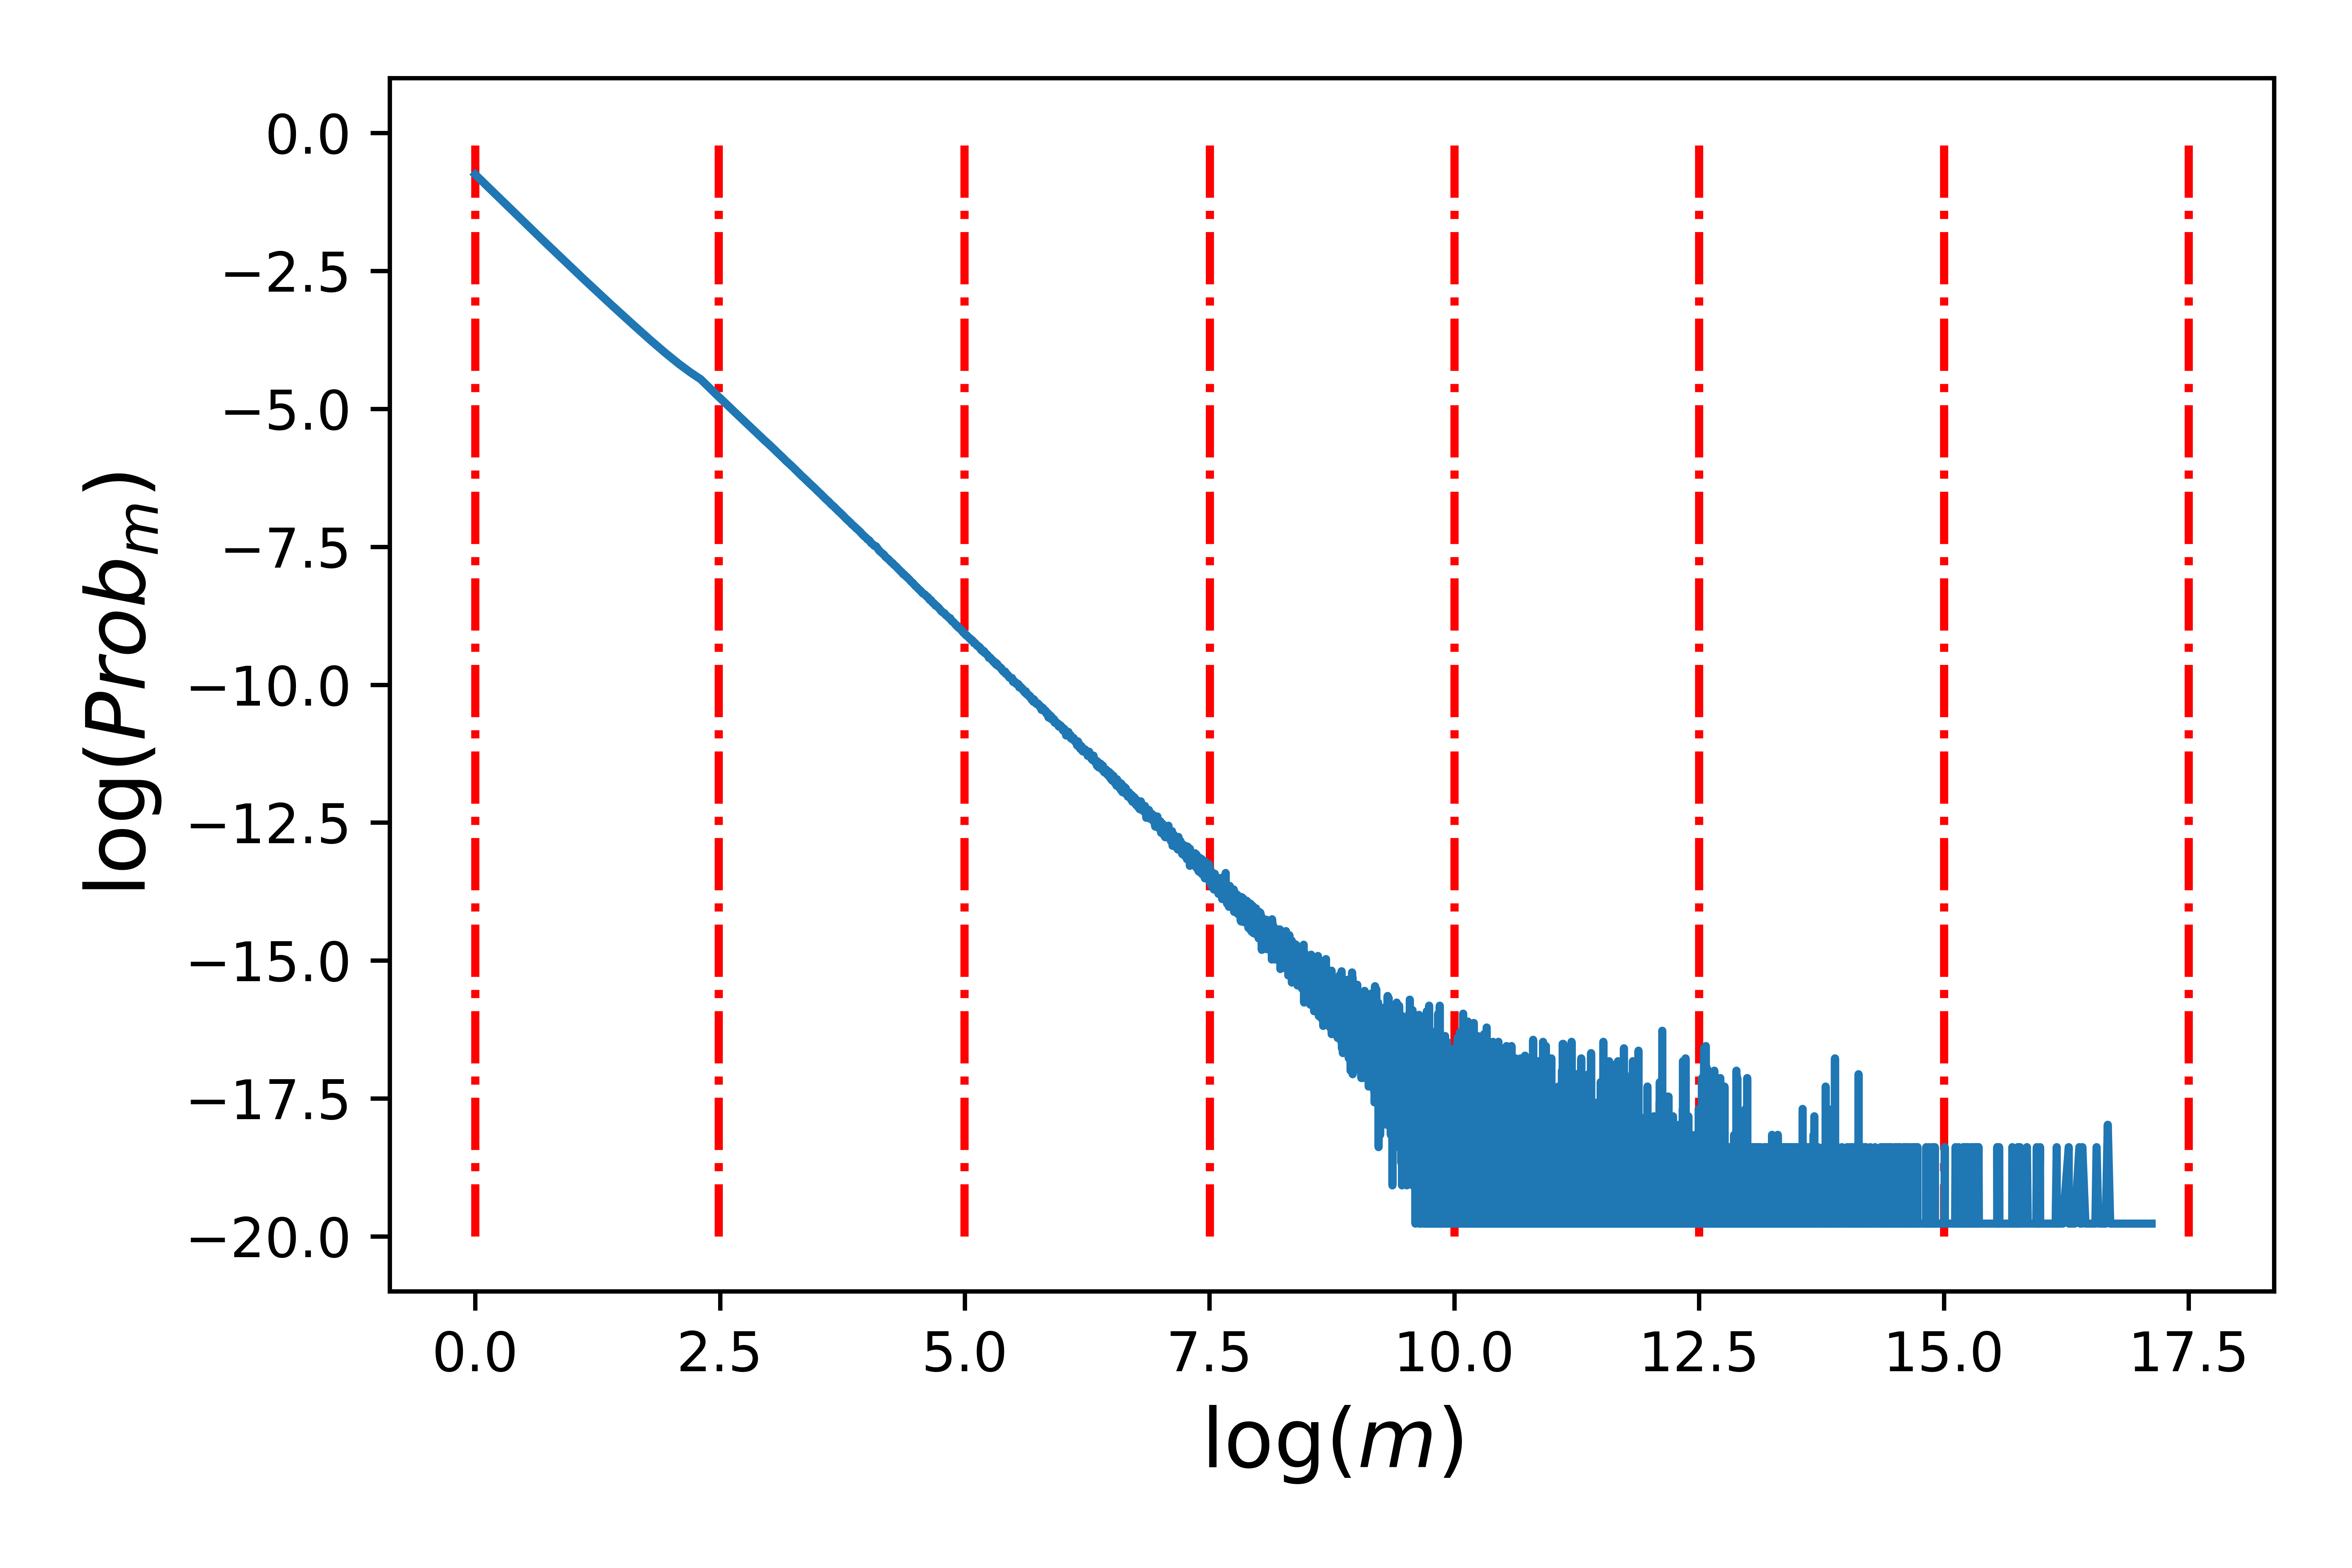
\includegraphics[width=0.5\textwidth]{criteo-thresh.png}
	\caption{Distribution of feature-pair frequency. Both axes are log-scaled. Vertical lines correspond to $val_{\text{thresh}}$ values used in Table.\ref{tab4}}
	\label{fig.1}
\end{figure}

From Figure \ref{fig.1}, $prob_{m}$ is larger when $m$ is small, indicating that many feature pairs occur a small number of times. This situation is reasonable because the set is very sparse. However, in the figure we observe that some pairs occur very frequently. For this set, dense and feature pairs can be well separated at around $\log(m)=10$. Interestingly, this cutting point corresponds to the smallest validation logloss in Table \ref{tab4}. Thus the validation procedure effectively finds a good $val_{\text{thresh}}$ to optimally combine Poly2 and FFM. To see if our method is equally effective for other data sets, in Figure \ref{fig.2}. we give the distribution of feature-pair frequencies for the other two sets, Avazu and Company. In the figure of each set, we draw a vertical line to indicate the $val_{\text{thresh}}$ that leads to the best validation logloss. Clearly, the obtained value rightly separates dense and sparse feature pairs. Then suitable models can be applied accordingly.

\begin{figure}
	\centering
	\subfigure[Avazu set]{
		\begin{minipage}[b]{0.5\textwidth}
			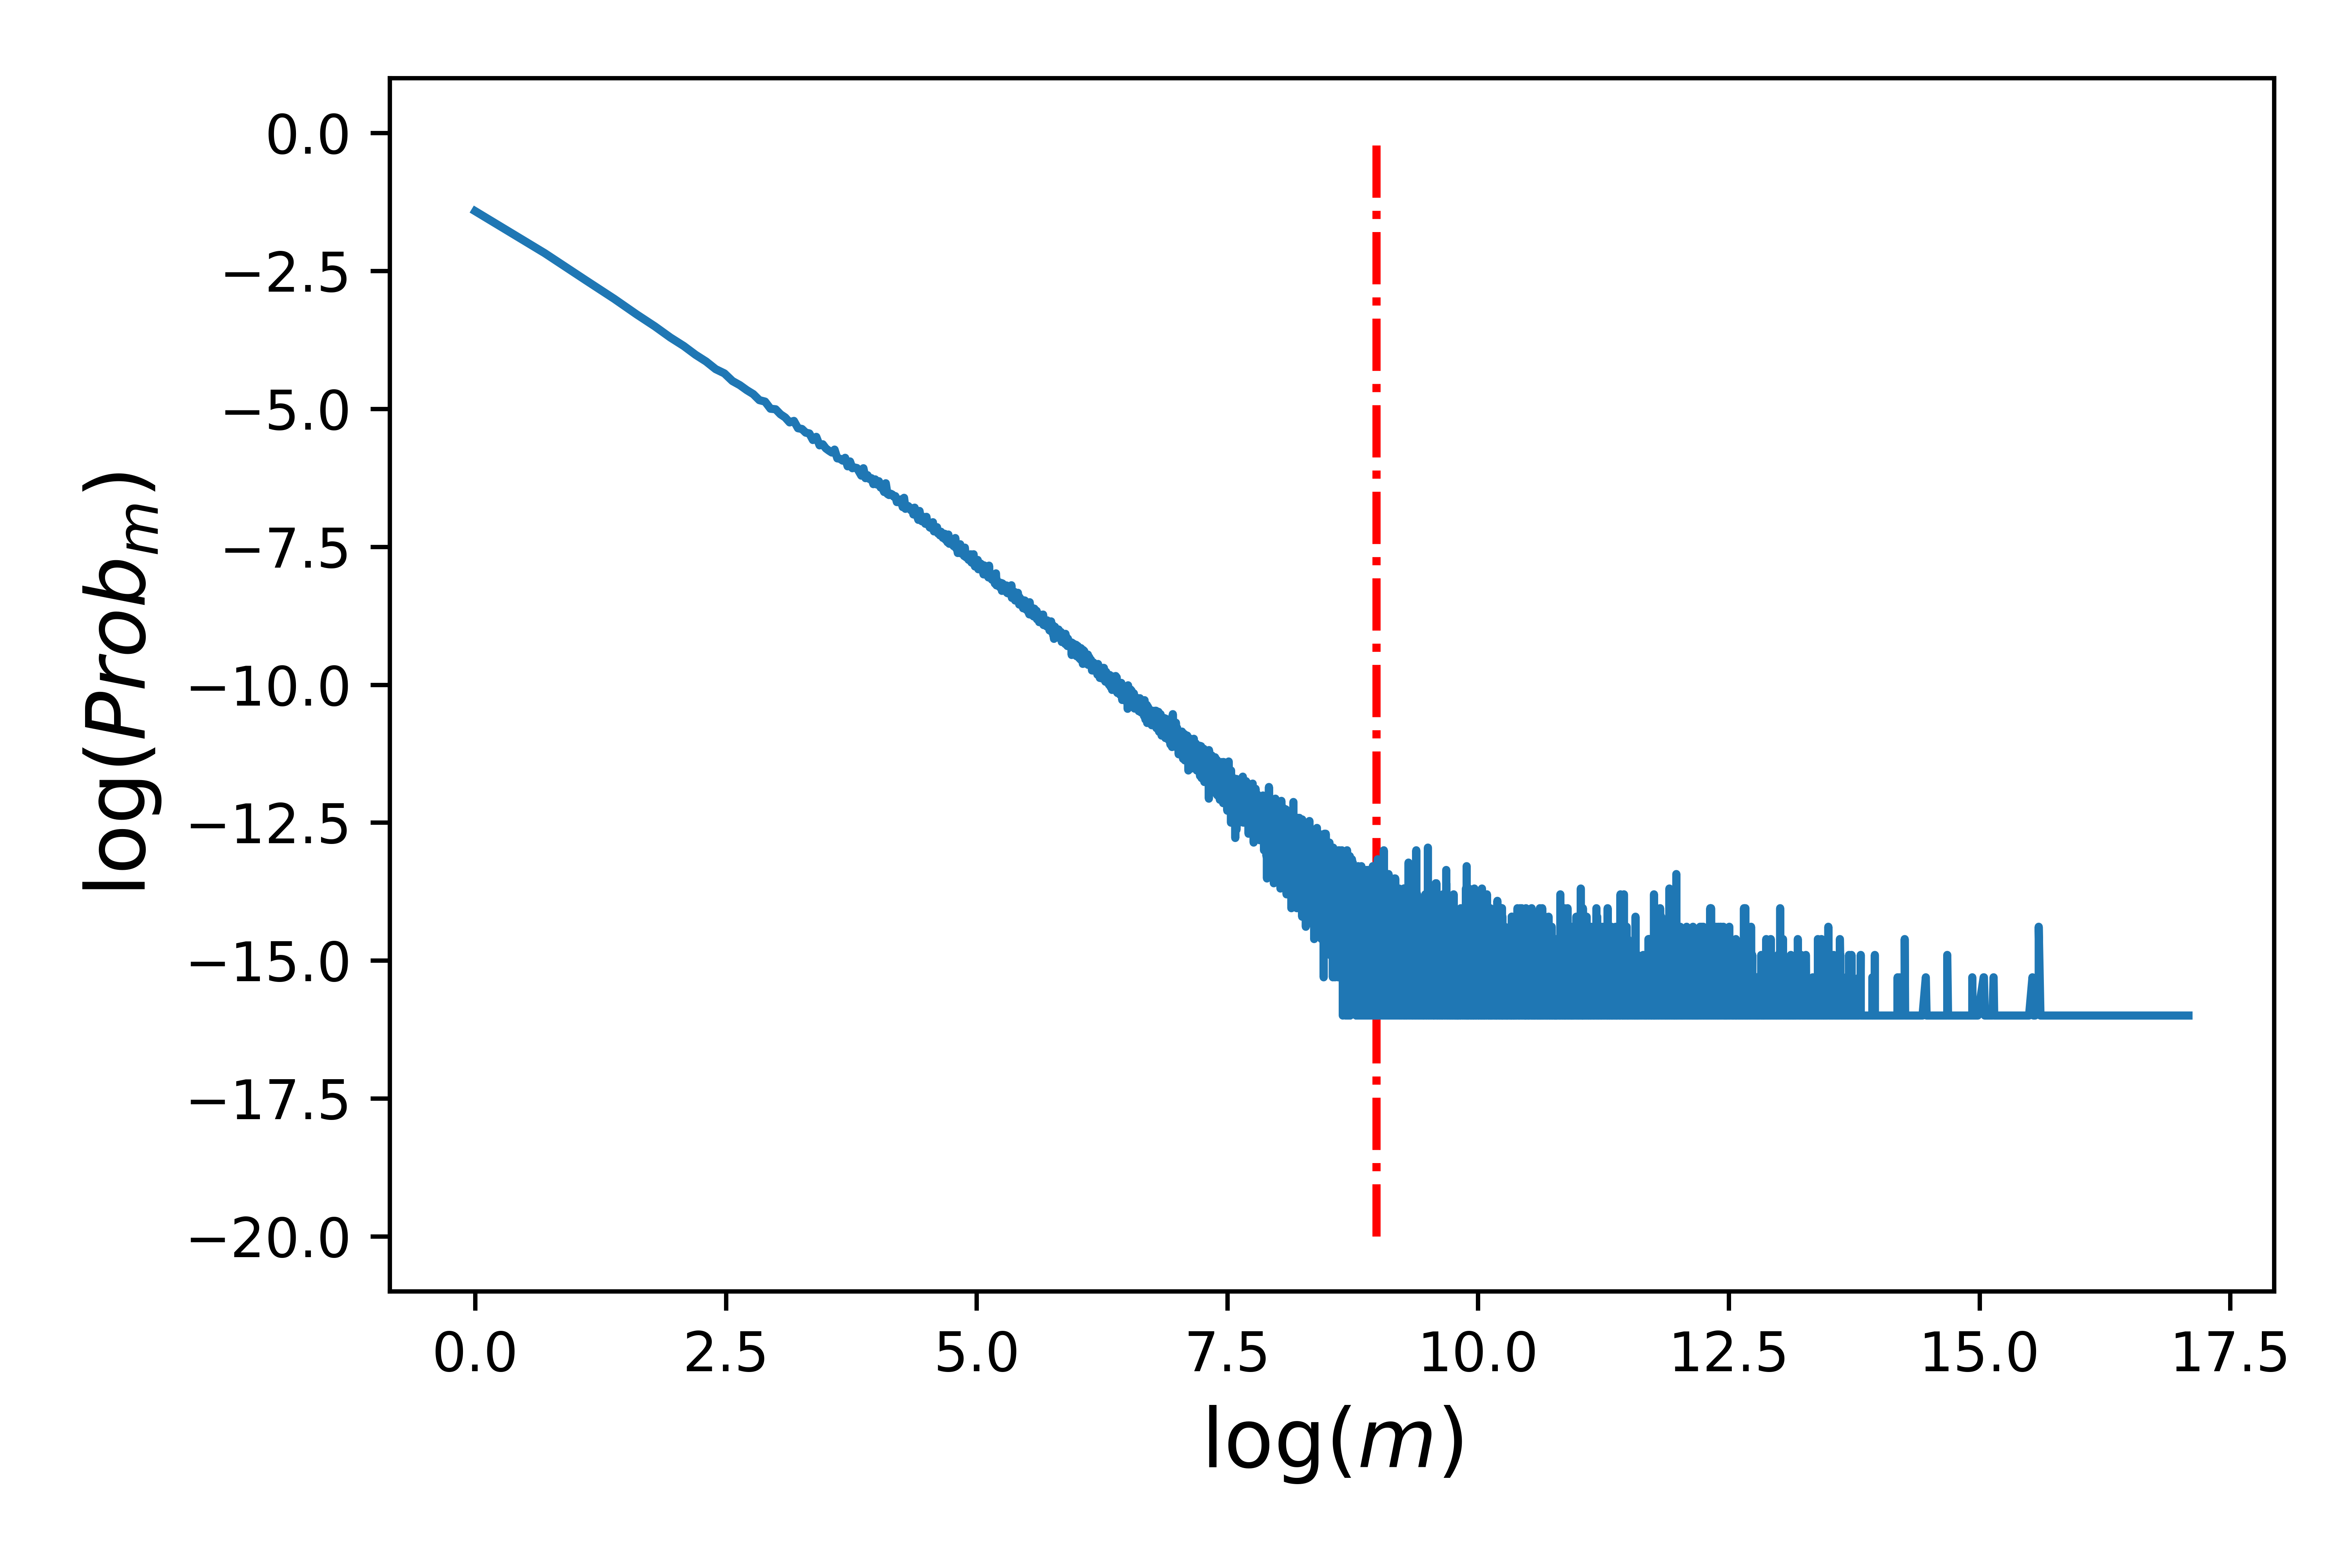
\includegraphics[width=1\textwidth]{avazu-thresh.png}
		\end{minipage}
	}
	\subfigure[Company set]{
	\begin{minipage}[b]{0.5\textwidth}
		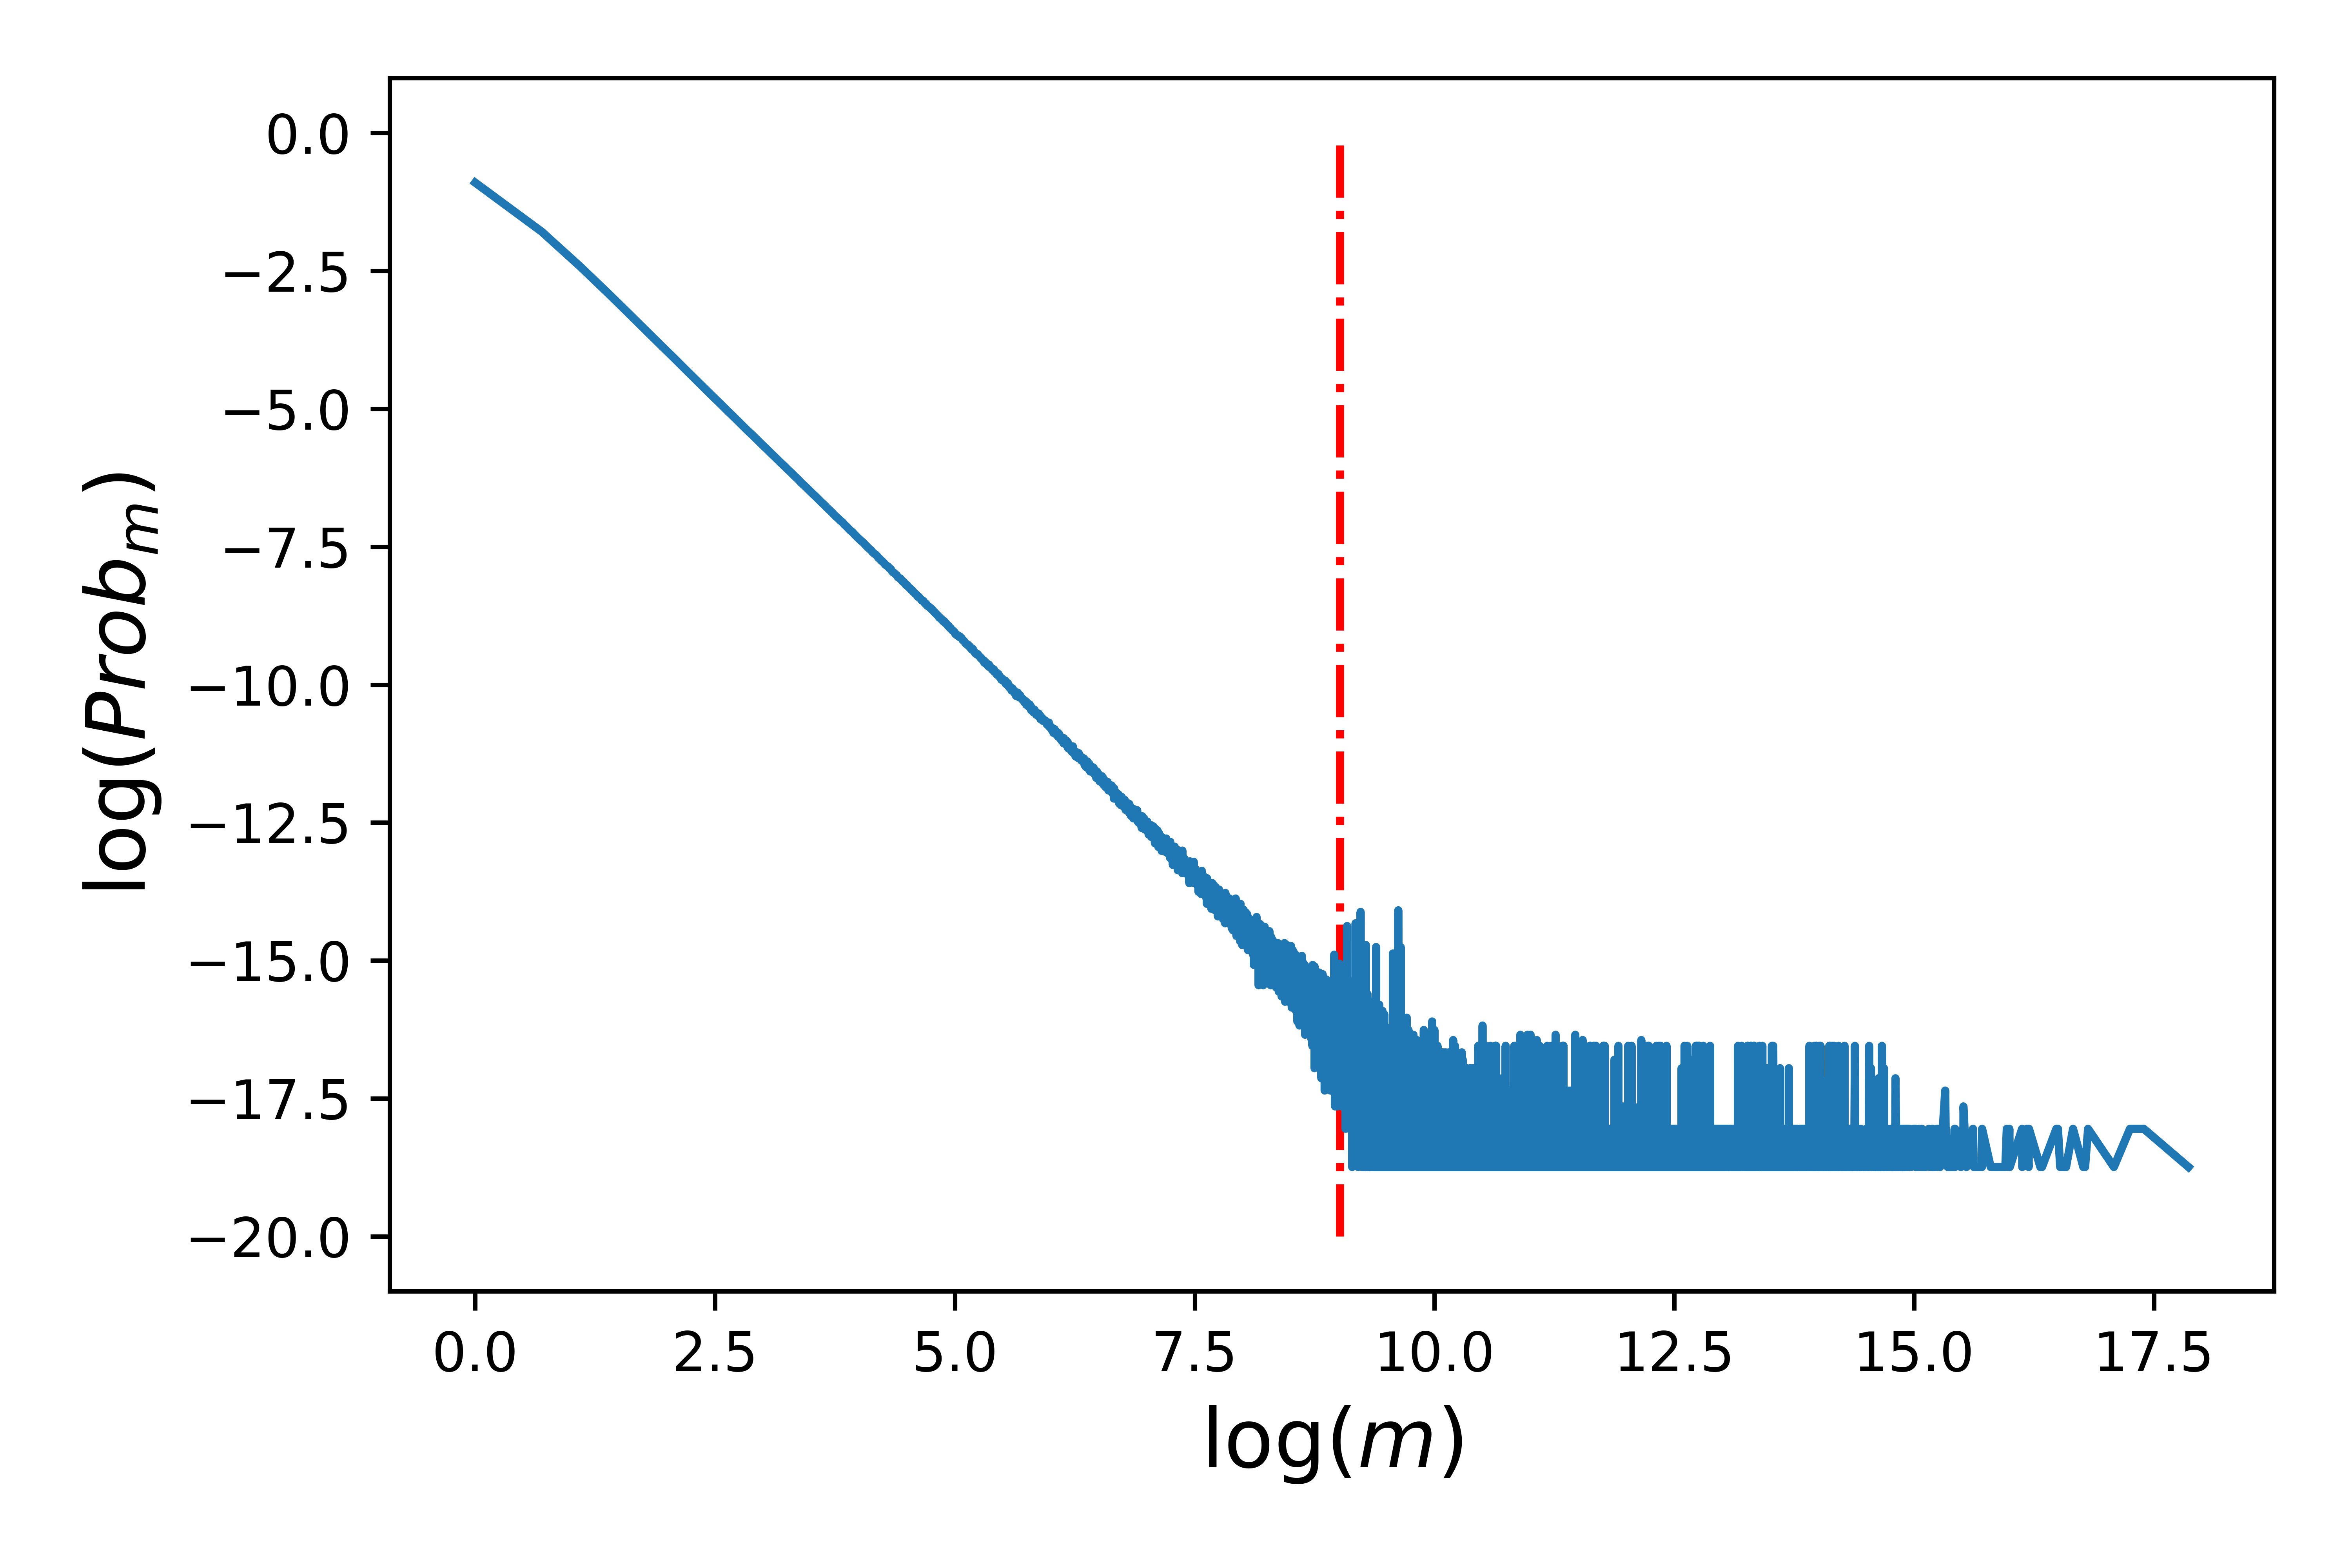
\includegraphics[width=1\textwidth]{hw-thresh.png}
	\end{minipage}}
	\caption{Distribution of feature-pair frequency of Avazu and Company sets. Both axes are log-scaled. Vertical lines correspond to the optimal $val_{\text{thresh}}$ values used in Table \ref{tab2}.}
	\label{fig.2}
\end{figure}
